\lstset{style=TigerJython, basicstyle=\scriptsize\ttfamily}
\begin{frame}[label=title]
    \centering
    \begin{figure}[H]
        
\includegraphics[keepaspectratio, width=0.7\paperwidth, height=\paperheight]{Logos/LeeLogo}
    \end{figure}
    Informatik: Data Science und Sicherheit\\
	\emoji{key} \textbf{Geheimschriften}
\end{frame}


\begin{frame}[label=schemakrypto]{Internet = \textit{offene} Technologie}
\begin{figure}[H]
\centering
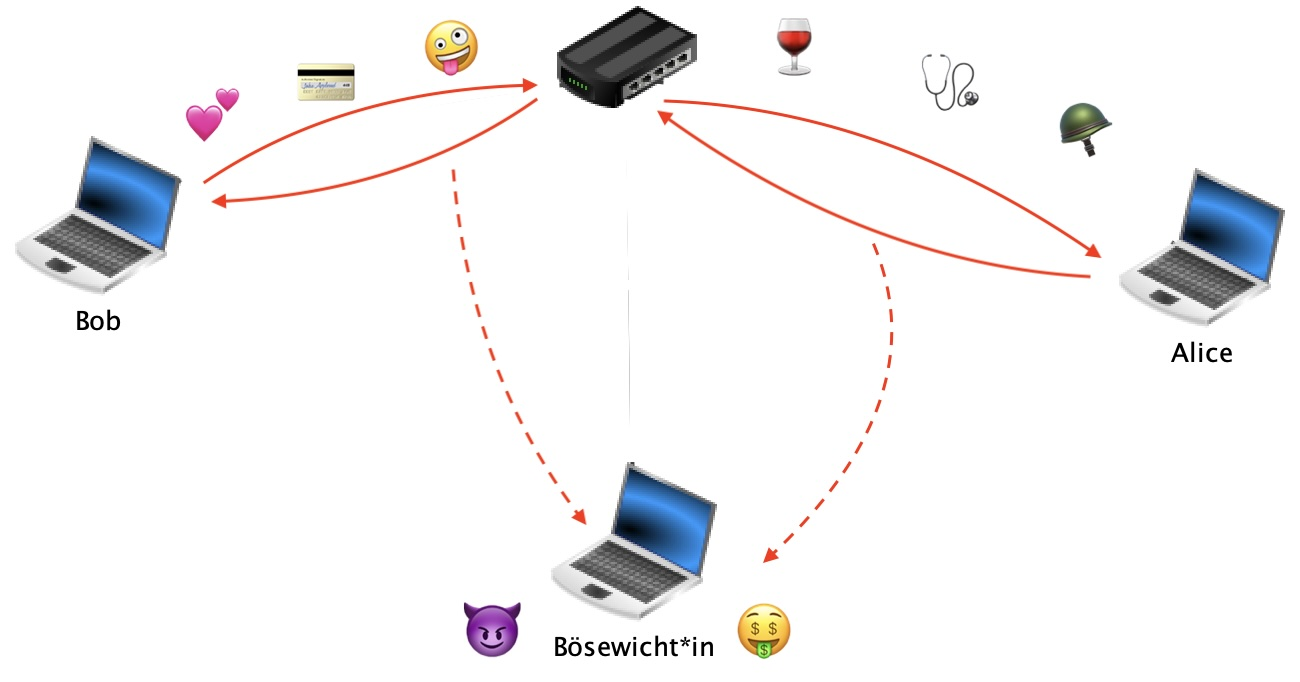
\includegraphics[width=\linewidth]{GrundlagenInfo/03_Kryptologie/Figures/filius-annotated}
\begin{center}
\only<1>{Was machen Sie alles im Internet?
}
\only<2>{
\large Z.B.: Sie schreiben eine Nachricht an Ihr \emoji{two-hearts}...\\
...und ich kann alles mitlesen! \emoji{teacher}}
\end{center}
\end{figure}

\end{frame}

\begin{frame}[label=schemakrypto]{Geheime Kommunikation zwischen Bob und Alice}
\begin{figure}
    \centering
    \begin{tikzpicture}[mylabel/.style={text width=20mm, align=center},scale=0.8, every node/.style={scale=0.8}]
    \node[bob, minimum width=1.5cm, 
        label={[mylabel, anchor=west]north east:{}}, 
        label={[mylabel, anchor=east]north west:{\textcolor{Blue}{Klartext} $\big\downarrow\text{\tiny (Verschlüsselung)}$\\
        \textcolor{Red}{Geheimtext}}}] (bob) {Bob (Sender)};
    \node[alice, minimum width=1.5cm, right=5cm of bob, mirrored,
        label={[mylabel, anchor=east]north west:{}}, 
        label={[mylabel, anchor=west]north east:{\textcolor{Red}{Geheimtext} $\big\downarrow\text{\tiny (Entschlüsselung)}$\\
        \textcolor{Blue}{Klartext}}}] (alice) {Alice (Empfänger)};
    
    \draw[->, thick, black] ([yshift=0mm]bob.east) coordinate(aux-a)-- coordinate[near start] (aux) node[above, text width=3cm, align=center]{\textcolor{Red}{Geheimtext}} (aux-a-|alice.west);

    \node[devil, minimum width=1.5cm, below right=13mm and 1.6cm of bob] (eve) {Eve (Gegner / Abhörer)};
    \draw[<-, gray] (eve)--(aux) node[midway,right]{abhören};
    \end{tikzpicture}
\end{figure}
\only<2->{\begin{tcolorbox}
\qrcode[height=1cm]{https://www.srf.ch/news/schweiz/cyberattacken-nehmen-zu-so-brutal-erpressen-hacker-schweizer-firmen} Würden Sie die Erpressungsgebühr zahlen?
\end{tcolorbox}}
\end{frame}


%\begin{frame}{Weshalb Verschlüsselung?}
%    \begin{figure}[H]
%        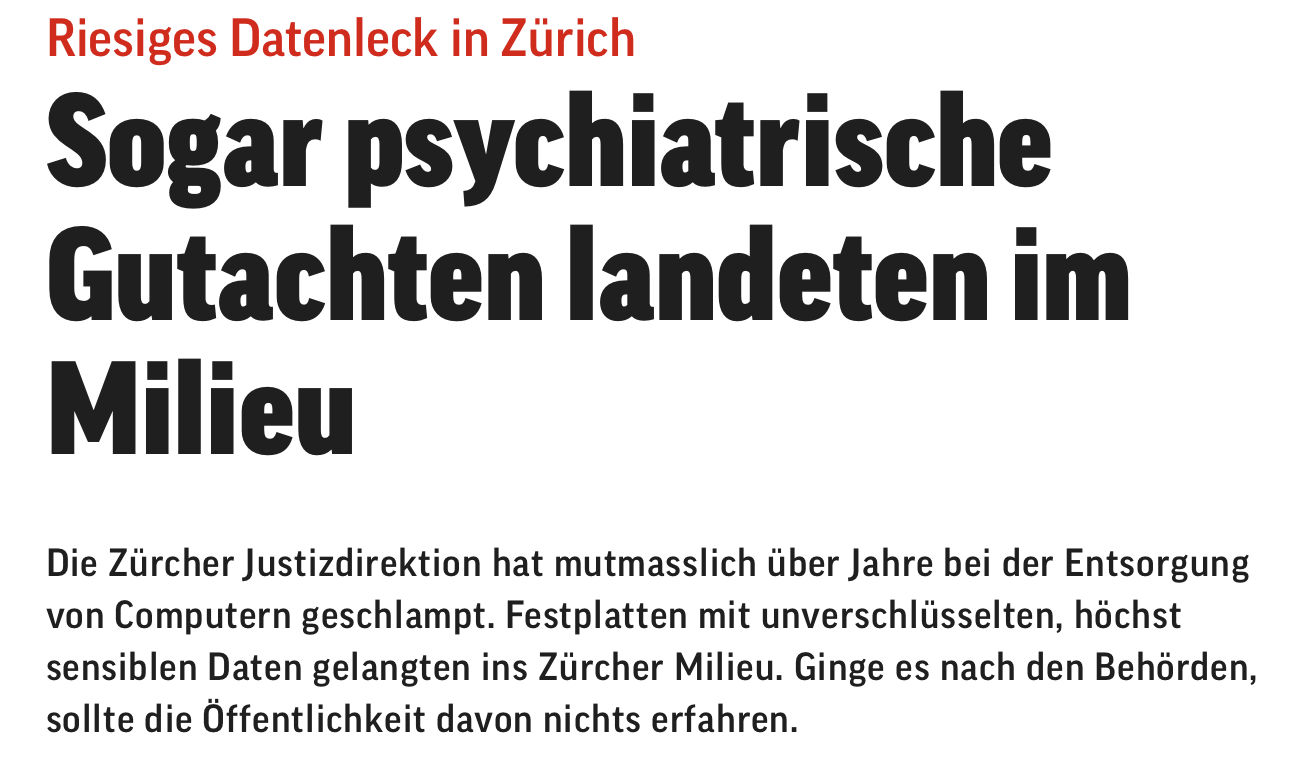
\includegraphics[keepaspectratio, width=0.49\linewidth]{GrundlagenInfo/03_Kryptologie/Figures/encryption-example-1.png}
%        \pause
%        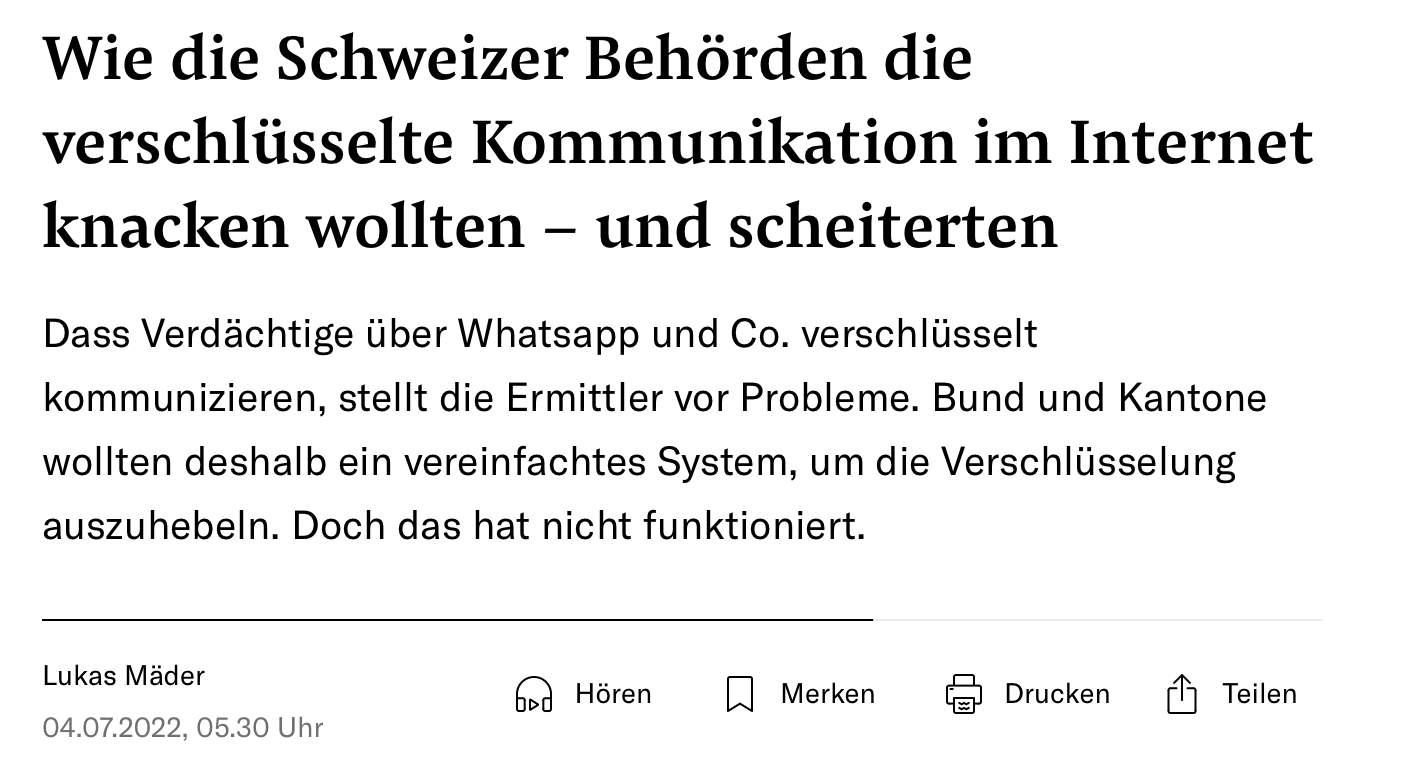
\includegraphics[keepaspectratio, width=0.49\linewidth]{GrundlagenInfo/03_Kryptologie/Figures/encryption-example-2.png}
%        \pause
%        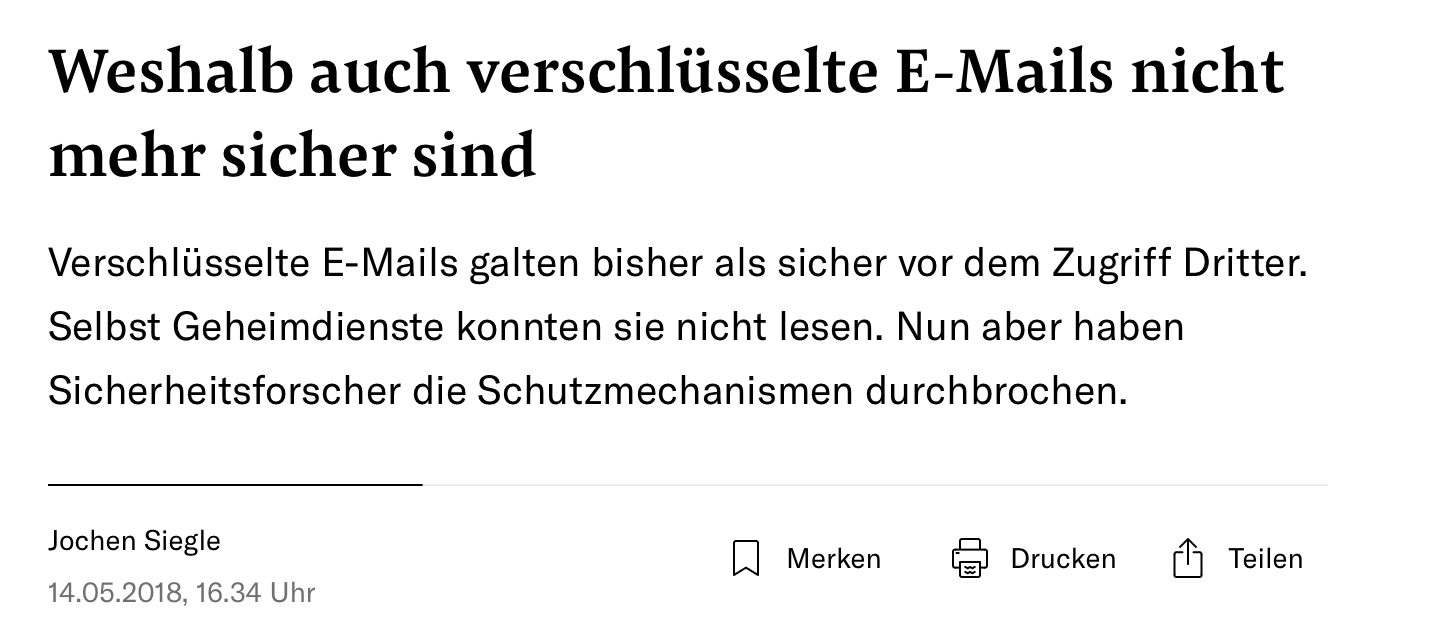
\includegraphics[keepaspectratio, width=0.6\linewidth]{GrundlagenInfo/03_Kryptologie/Figures/encryption-example-3.png}
%    \end{figure}
%\end{frame}

\begin{frame}{Kerkhoffs'sches Prinzip der Sicherheit}
\begin{figure}[H]
\centering
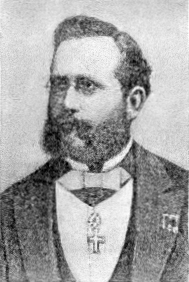
\includegraphics[width=0.3\linewidth]{GrundlagenInfo/03_Kryptologie/Figures/kerckhoffs}
\end{figure}
\begin{quote}
``Il faut qu’il n’exige pas le secret, et qu’il puisse sans inconvénient tomber entre les mains de l’ennemi.'' \\
-- Auguste Kerckhoffs, \textit{La cryptographie militaire} (1883)
\end{quote}
\begin{center}
\only<2->{Kein Geheimhaltung $\rightarrow$ \textbf{Open Source}!}
\end{center}
\end{frame}

\begin{frame}{Anforderungen an kryptographische Systeme}
\begin{enumerate}[<+->]
    \item \textbf{Vertraulichkeit}: Es soll sichergestellt sein, dass wirklich nur diejenige eine Nachricht lesen kann, für die diese bestimmt ist.
    \item \textbf{Integrität}: Die Empfängerin soll feststellen können, ob die Nachricht nach ihrer Erzeugung verändert wurde.
    \item \textbf{Authentizität}: Der Verfasser einer Nachricht soll identifizierbar sein, bzw. die Empfängerin soll nachprüfen können, wer der Verfasser ist.
    \item \textbf{Verbindlichkeit}: Der Verfasser soll nicht abstreiten können, dass er der Verfasser der Nachricht ist.
\end{enumerate}
\end{frame}

\begin{frame}{Symmetrische Verschlüsselungsverfahren}
    \begin{itemize}[<+->]
        \item \emoji{key} Derselbe \textbf{Schlüssel} zur Ver- und Entschlüsselung
        \item \emoji{shushing-face} Sender und Empfänger müssen sich auf einen Schlüssel einigen, ohne dass ein Dritter mithören kann
        \item \emoji{locked-with-key} Analogie: Schatzkiste versenden
    \end{itemize}

\end{frame}

\begin{frame}[label=intro1]{Einführungsaufgabe 1}
    Der Geheimtext lautet:
    \begin{center}
        AMEHT SEGITHCIW NIE TSI EIGOLOTPYRK
    \end{center}
    Stellen Sie den ursprünglichen Text wieder her.
\end{frame}

\begin{frame}[label=intro1Sol]{Lösung der Einführungsaufgabe 1}
    \begin{center}
    
        Geheimtext:\\
        AMEHT SEGITHCIW NIE TSI EIGOLOTPYRK\\
        \bigskip
        ursprünglicher Text:\\
        KRYPTOLOGIE IST EIN WICHTIGES THEMA\\
    \end{center}
    Der Geheimtext entspricht dem von rechts nach links (rückwärts) gelesenen ursprünglichen Text.
\end{frame}

\begin{frame}[label=intro2]{Einführungsaufgabe 2}
    Der Geheimtext lautet:
    \begin{center}
    \small
        \begin{enumerate}
            \item RKPYOTOLIGEEMREOLGCITHEGEHMIINSSE
            \item HCSFIRILTAHCZFUEBUHAWNERDNUKUZMMOINUEIZNER
        \end{enumerate}
        \normalsize
    \end{center}
    Stellen Sie den ursprünglichen Text wieder her.
\end{frame}

\begin{frame}[label=intro2Sol]{Lösung Einführungsaufgabe 2}
    Geheimtext:
    \begin{center}
    \small
        \begin{enumerate}
            \item RKPYOTOLIGEEMREOLGCITHEGEHMIINSSE
            \item HCSFIRILTAHCZFUEBUHAWNERDNUKUZMMOINUEIZNER
        \end{enumerate}
        \normalsize
    \end{center}
    Ursprünglicher Text:
    \begin{center}
    \small
        \begin{enumerate}
            \item KRYPTOLOGIE ERMOEGLICHT GEHEIMNISSE
            \item SCHRIFTLICH AUFZUBEWAHREN UND ZU KOMMUNIZIEREN
        \end{enumerate}
        \normalsize
    \end{center}
    Der Geheimtext entsteht durch Austauschen der Positionen der Buchstaben.
    \begin{figure}[H]
        \centering
        \begin{subfigure}[b]{0.45\textwidth}
          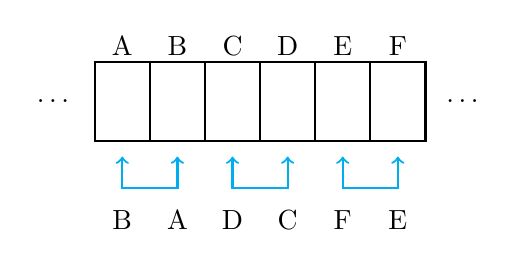
\begin{tikzpicture}
              % Parameters
              \def\boxwidth{.7} % Width of each box
              \def\numboxes{6} % Total number of boxes
              \pgfmathtruncatemacro{\lastindex}{\numboxes-2} % Compute the last valid index for swapping
              \pgfmathtruncatemacro{\lastindexLet}{\numboxes-1} % Compute the last valid index for swapping
              
          
              % Draw the rectangle (sequence of letters)
              \draw[thick] (0, 0) rectangle (\numboxes*\boxwidth, 1);
              \foreach \i in {1,...,\numboxes} {
                  \draw[thick] (\i*\boxwidth, 0) -- (\i*\boxwidth, 1);
              }
          
              % Add ellipses on both sides
              \node at (-0.5, 0.5) {\dots};
              \node at (\numboxes*\boxwidth+0.5, 0.5) {\dots};
          
              % Add arrows for swapping
              \foreach \i in {0,2,...,\lastindex} {
                  \pgfmathsetmacro{\xstart}{\i*\boxwidth + 0.5*\boxwidth}
                  \pgfmathsetmacro{\xend}{\xstart + \boxwidth}
                  \draw[thick, cyan, <->] (\xstart, -0.2) -- (\xstart, -0.6) -- (\xend, -0.6) -- (\xend, -0.2);
              }
          
              % Add letters above the boxes
              \foreach \i in {0,...,\lastindexLet} {
                  \pgfmathsetmacro{\xpos}{\i*\boxwidth + 0.5*\boxwidth}
                  \pgfmathtruncatemacro{\letter}{65+\i} % ASCII value of A is 65
                  \node at (\xpos, 1.2) {\char\letter};
              }
          
              % Add swapped letters below the boxes
              \foreach \i in {0,...,\lastindexLet} {
                  \pgfmathsetmacro{\xpos}{\i*\boxwidth + 0.5*\boxwidth}
                  \ifodd\i
          	        \pgfmathtruncatemacro{\swapletter}{65+\i-1} % ASCII value of A is 65
                  \else
                      \pgfmathtruncatemacro{\swapletter}{65+\i+1} % ASCII value of A is 65
                  \fi
                  \node at (\xpos, -1) {\char\swapletter};
              }
          \end{tikzpicture}
          \caption{\enquote{Zweiertausch}}
        \end{subfigure}
        \hfill
        \begin{subfigure}[b]{0.45\textwidth}
          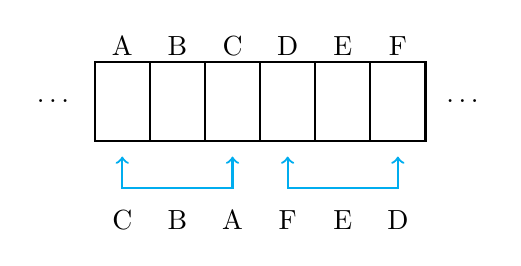
\begin{tikzpicture}
              % Parameters
              \def\boxwidth{.7} % Width of each box
              \def\numboxes{6} % Total number of boxes
              \pgfmathtruncatemacro{\lastindex}{\numboxes-3} % Compute the last valid index for swapping
              \pgfmathtruncatemacro{\lastindexLet}{\numboxes-1} % Compute the last valid index for swapping
              
          
              % Draw the rectangle (sequence of letters)
              \draw[thick] (0, 0) rectangle (\numboxes*\boxwidth, 1);
              \foreach \i in {1,...,\numboxes} {
                  \draw[thick] (\i*\boxwidth, 0) -- (\i*\boxwidth, 1);
              }
          
              % Add ellipses on both sides
              \node at (-0.5, 0.5) {\dots};
              \node at (\numboxes*\boxwidth+0.5, 0.5) {\dots};
          
              % Add arrows for swapping
              \foreach \i in {0,3,...,\lastindex} {
                  \pgfmathsetmacro{\xstart}{\i*\boxwidth + 0.5*\boxwidth}
                  \pgfmathsetmacro{\xend}{\xstart + \boxwidth*2}
                  \draw[thick, cyan, <->] (\xstart, -0.2) -- (\xstart, -0.6) -- (\xend, -0.6) -- (\xend, -0.2);
              }
          
              % Add letters above the boxes
              \foreach \i in {0,...,\lastindexLet} {
                  \pgfmathsetmacro{\xpos}{\i*\boxwidth + 0.5*\boxwidth}
                  \pgfmathtruncatemacro{\letter}{65+\i} % ASCII value of A is 65
                  \node at (\xpos, 1.2) {\char\letter};
              }
          
              % Add swapped letters below the boxes
              \foreach \i in {0,3,...,\lastindex} {
          	    \pgfmathtruncatemacro{\swapletter}{65+\i+2} % ASCII value of A is 65
          	    \pgfmathsetmacro{\xpos}{\i*\boxwidth + 0.5*\boxwidth}
                  \node at (\xpos, -1) {\char\swapletter};
              }
              
              \foreach \i in {2,5,...,\numboxes} {
          	    \pgfmathtruncatemacro{\swapletter}{65+\i-2} % ASCII value of A is 65
          	    \pgfmathsetmacro{\xpos}{\i*\boxwidth + 0.5*\boxwidth}
                  \node at (\xpos, -1) {\char\swapletter};
              }
              
              \foreach \i in {1,4,...,\lastindexLet} {
          	    \pgfmathtruncatemacro{\swapletter}{65+\i} % ASCII value of A is 65
          	    \pgfmathsetmacro{\xpos}{\i*\boxwidth + 0.5*\boxwidth}
                  \node at (\xpos, -1) {\char\swapletter};
              }
          \end{tikzpicture}
          \caption{\enquote{Dreiertausch}}
        \end{subfigure}
    \end{figure}
\end{frame}


\section{Chiffrierung mithilfe von Tabellen}

\begin{frame}{Stock-und-Streifen-Verschlüsselung}
\begin{center}
\large \emoji{jigsaw} Wer löst das Rätsel zuerst?
\end{center}
\end{frame}

\begin{frame}{Stock-und-Streifen-Verschlüsselung}
\begin{figure}
\centering
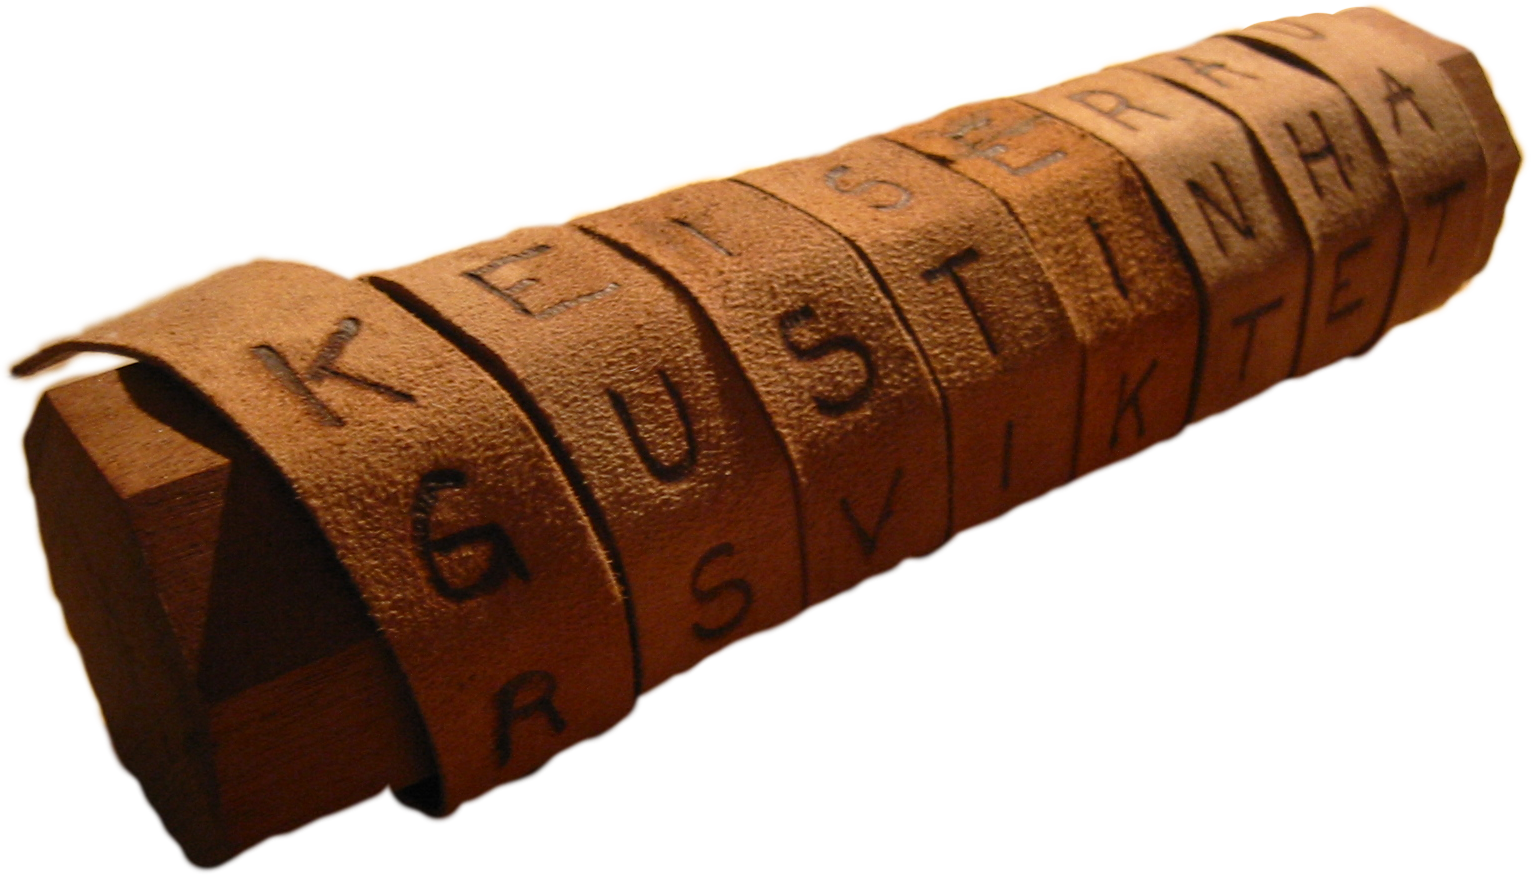
\includegraphics[width=0.7\linewidth]{GrundlagenInfo/03_Kryptologie/Figures/SkytaleWiki}
\end{figure}
$\rightarrow$ \textbf{Skytale} (von altgriechisch \textit{skytálē} = ``Stock'', ``Stab'')
\begin{itemize}[<+->]
\item Ältestes bekanntes militärisches Verschlüsselungsmethode der Welt!
\item Von Spartanern vor 2500 Jahren verwendet
\end{itemize}
\end{frame}

\begin{frame}[label=skytale1]{Skytale}
\begin{itemize}
    \item Schreibe den Klartext zeilenweise in eine Tabelle (Matrix) von links nach rechts.
    \item Der Geheimtext erhalten wir, indem wir die Buchstaben Spalte für Spalte von links nach rechts lesen.
\end{itemize}
\begin{table}[]
\begin{tabular}{|c|c|c|c|c|c|c|}
\hline
\blue{S} & P & A & R & T & A & \blue{W} \\ \hline
A & R & \blue{I} & N & \blue{D} & E & R \\ \hline
\blue{A} & N & T & I & K & E & \blue{D} \\ \hline
E & R & \blue{H} & A & U & P & T \\ \hline
O & R & T & \blue{D} & E & R & \blue{L} \\ \hline
A & N & D & S & C & H & A \\ \hline
F & T & \blue{L} & A & K & O & N \\ \hline
I & E & N & \red{X} & \red{K} & \red{M} & \red{G} \\ \hline
\end{tabular}
\end{table}
\end{frame}

\begin{frame}[label=skytale2]{Skytale}
\begin{itemize}
    \item Falls der Klartext die Tabelle nicht vollständig ausfüllt, so füllt man die leeren Felder mit beliebigen Buchstaben auf (rot markiert).
\end{itemize}
\begin{table}[]
\begin{tabular}{|c|c|c|c|c|c|c|}
\hline
\blue{S} & P & A & R & T & A & \blue{W} \\ \hline
A & R & \blue{I} & N & \blue{D} & E & R \\ \hline
\blue{A} & N & T & I & K & E & \blue{D} \\ \hline
E & R & \blue{H} & A & U & P & T \\ \hline
O & R & T & \blue{D} & E & R & \blue{L} \\ \hline
A & N & D & S & C & H & A \\ \hline
F & T & \blue{L} & A & K & O & N \\ \hline
I & E & N & \red{X} & \red{K} & \red{M} & \red{G} \\ \hline
\end{tabular}
\end{table}
\end{frame}

%\begin{frame}[label=skytaleEx1]{SKYTALE Aufgabe 1}
%Die Geheimschrift
%\begin{center}
%    WNGIAEIEMATSMKRTTEAGIEINANINTUGNDOJEEENL
%\end{center}
%wurde mit einer Tabelle mit 5 Zeilen und 8 Spalten erzeugt. Wie lautet der Klartext?
%\end{frame}

%\begin{frame}[label=skytaleEx1Sol]{Lösung SKYTALE Aufgabe 1}
%Wir beginnen mit einer leeren $5\times 8$ Tabelle und schreiben den Geheimtext spaltenweise (von rechts nach links und von oben nach unten) in die leere Tabelle. Damit erhalten wir:
%\begin{table}[]
%\begin{tabular}{|c|c|c|c|c|c|c|c|}
%\hline
%W & E & T & T & I & N & G & E \\ \hline
%N & I & S & T & E & I & N & E \\ \hline
%G & E & M & E & I & N & D & E \\ \hline
%I & M & K & A & N & T & O & N \\ \hline
%A & A & R & G & A & U & \red{J} & \red{L} \\ \hline
%\end{tabular}
%\end{table}
%Der Klartext
%\begin{center}
%    Wettingen ist eine Gemeinde im Kanton Aargau
%\end{center}
%lässt sich nun einfach ablesen.
%\end{frame}

%\begin{frame}[label=skytaleEx2]{SKYTALE Aufgabe 2}
%Sie möchten einen Klartext der Länge 87 mit Hilfe einer Tabelle mit 10 Zeilen chiffrieren. Wie viele Spalten benötigt diese Tabelle?
%\end{frame}
%
%\begin{frame}[label=skytaleEx2Sol]{Lösung SKYTALE Aufgabe 2}
%Die Tabelle benötigt 9 Spalten. Allgemein lässt sich die Anzahl benötigter Spalten berechnen durch
%\begin{align*}
%    \ceil{\frac{\text{Länge des Textes}}{\text{Anzahl Zeilen}}}\quad\text{(nach oben aufgerundet)}.
%\end{align*}
%\end{frame}
%
%\begin{frame}[label=skytaleEx3]{SKYTALE Aufgabe 3}
%Der folgende Geheimtext der Länge 75 wurde mit SKYTALE verschlüsselt:
%\begin{center}
%ETIFIITNUTNFGENKURRELEODIERSILIMSEANIE\\
%MRECREMRHSNSSAPSTCBRCRHEUHORRNHNIEGEG 
%\end{center}
%Dabei konnten \textbf{alle Zeilen der Tabelle vollständig aufgefüllt} werden.
%\begin{description}
%\item[(a)] Welches ist hier der Schlüssel (die Anzahl der Zeilen)? Tipp: Probieren Sie die Schlüssel 3 und 5 aus.
%\item[(b)] Wie lautet der Klartext?
%\item[(c)] Wie viele Schlüssel müssen im schlimmsten Fall ausprobiert werden, bis der korrekte Schlüssel gefunden wurde? Das heisst, wie viele potentielle Schlüssel gibt es?
%\end{description}
%\end{frame}

%\begin{frame}[fragile, label=skytaleEx3Sol]{Lösung SKYTALE Aufgabe 3}
%% \adjustbox{width=0.7\textwidth}{%
%\begin{table}[]
%\begin{tabular}{|c|c|c|c|c|c|c|c|c|c|c|c|c|c|c|}
%\hline
%E & I & N & K & L & E & I & N & E & R & S & C & H & R & I \\ \hline
%T & T & F & U & E & R & M & I & C & H & A & B & E & R & E \\ \hline
%I & N & G & R & O & S & S & E & R & S & P & R & U & N & G \\ \hline
%F & U & E & R & D & I & E & M & E & N & S & C & H & H & E \\ \hline
%I & T & N & E & I & L & A & R & M & S & T & R & O & N & G \\ \hline
%\end{tabular}
%\end{table}
%% }%
%\begin{description}
%\item[(a)] Durch Ausprobieren finden wir, dass die Wahl des Schlüssels 5 zu einem sinnvollen Klartext führt, die Wahl des Schlüssels 3 jedoch nicht.
%
%\item[(b)]
%Der Klartext lautet also:
%\begin{center}
%    {\small
%    EIN KLEINER SCHRITT FUER MICH ABER EIN GROSSER\\
%    SPRUNG FUER DIE MENSCHHEIT NEIL ARMSTRONG}
%\end{center}
%\item[(c)] Wir müssen $75=3\cdot 5\cdot 5$ Buchstaben auf ein Rechteck verteilen. Damit könnten $3, 5, 15$ und $25$ mögliche Schlüssel sein. $1$ und $75$ sind keine Schlüssel, da der gegebene Text kein Klartext ist.
%\end{description}
%\end{frame}

%\begin{frame}[fragile]{Auftrag Halbklassen (Programmieren)}
%\begin{itemize}
%\item \abgabebox{Aufgabe 1.2}
%\end{itemize}
%\textbf{Tipp}: Bei Unklarheiten, schauen Sie das Skript zu Zeichneketten an!
%\end{frame}

\begin{frame}[fragile]{Auftrag}
Skript (auf Moodle)
\begin{itemize}
\item \aufgabebox{Aufgaben 1.2, 1.3}
\item \challengebox{Aufgabe 1.4}
\end{itemize}
\end{frame}

\begin{frame}{Zeichen Ersetzen}
\begin{center}
Welche Methoden kennen wir bereits?
\end{center}
\end{frame}

\begin{frame}[fragile]{ASCII (Auszug)}
\begin{table}[H]
	\centering
	\tiny
	\begin{tabular}{cccc}
		\toprule
		Dezimal & Hexadezimal & Binär & Zeichen \\
		\midrule
		0 & 00 & 00000000 & NUL \\
		1 & 01 & 00000001 & SOH \\
		2 & 02 & 00000010 & STX \\
		3 & 03 & 00000011 & ETX \\
		4 & 04 & 00000100 & EOT \\\midrule
		... & ... & ... & ... \\\midrule
		36 & 24 & 00100100 & \$ \\
		37 & 25 & 00100101 & \% \\
		38 & 26 & 00100110 & \& \\
		39 & 27 & 00100111 & ' \\
		40 & 28 & 00101000 & ( \\
		41 & 29 & 00101001 & ) \\\midrule
		... & ... & ... & ... \\\midrule
		48 & 30 & 00110000 & 0 \\
		49 & 31 & 00110001 & 1 \\
		50 & 32 & 00110010 & 2 \\
		51 & 33 & 00110011 & 3 \\
		52 & 34 & 00110100 & 4 \\\midrule
		... & ... & ... & ... \\\midrule
		65 & 41 & 01000001 & A \\
		66 & 42 & 01000010 & B \\
		67 & 43 & 01000011 & C \\
		68 & 44 & 01000100 & D \\
		69 & 45 & 01000101 & E \\\midrule
		... & ... & ... & ... \\\bottomrule
	\end{tabular}
\end{table}
\end{frame}

\begin{frame}[label=caesar]{Caesar-Kryptosystem \emoji{amphora}}
    \begin{minipage}[c]{.45\linewidth}
    \begin{itemize}
        \item Zwei Drehscheiben: Klartext aussen, Geheimtext innen
        \item Schlüssel = Verschiebung der inneren Scheibe gegenüber A
        \item Z.B.: HALLO = KDOOR
        \item Extrem unsichere Verschlüsselung: Nur 26 mögliche Schlüssel
    \end{itemize}
    \end{minipage}
    \begin{minipage}[c]{.45\linewidth}
        \begin{figure}[H]
        \centering
        \resizebox{\linewidth}{!}{\caesar[3]}
    \end{figure}
    \end{minipage}
\end{frame}

\begin{frame}[fragile]{Auftrag}
Skript (auf Moodle)
\begin{itemize}
\item \aufgabebox{Aufgaben 1.5, 1.6}
\end{itemize}
\end{frame}

\begin{frame}[label=caesarex, fragile]{Angriff auf Caesar}
	\centering
	Wie würden Sie folgenden Text knacken?\\[.5cm]
	    \defverbatim{\verbOne}{
\small\begin{verbatim}
Geheimtext: PKSGTJSAYYZKPUYKLQBKXRKASJKZNG...
\end{verbatim}
	        }
 \defverbatim{\verbTwo}{
	      \small\begin{verbatim}
  Klartext: JEMANDMUSSTEJOSEFKVERLEUMDETHA...
 Schlüssel: GGGGGGGGGGGGGGGGGGGGGGGGGGGGGG...
Geheimtext: PKSGTJSAYYZKPUYKLQBKXRKASJKZNG...
	      \end{verbatim}
	      }
	    \only<1-5>{\verbOne}
	    \only<2-4>{
	    Häufigster Buchstabe im obigen Geheimtext: \texttt{K}\\
	    Häufigster Buchstabe im deutschen Alphabet: \texttt{E}
	    }
	    
	 \only<3-5>{
	 \begin{itemize}
	   \item<3-5> \texttt{E}: Buchstabe mit Ordnung 4
	   \item<4-5> \texttt{K}: Buchstabe mit Ordnung 10
	   \item<5> Schlüssel $=$ Verschiebung von $10-4= 6 =$ Buchstabe \texttt{G}
	 \end{itemize}	 
	 }
	 \only<5-6>{
	 \centering\scalebox{.6}{\caesar[6]}
	 }
	 
	 \only<6>{\verbTwo}	
\end{frame}

% \begin{frame}[label=auftrag]{Auftrag}
% \begin{itemize}
%     \item \emoji{pen} Lesen Sie den Inhalt der Box ``Neue Konzepte und Begriffe'' auf Moodle.
%     \item Lösen Sie die nachfolgenden Aufgaben. % TODO
%     \item Aufgabe 2.16 (Tipp: Drehscheibe verwenden)
%     \item Aufgabe 2.22
%     \item Lösen Sie die Aufgabe ``Geheimtext (Skytale)'' auf Moodle
%     \item \emoji{trophy} Challenge: 
%     \begin{itemize}
%         \item Aufgabe 2.2 (\emoji{snake} Python)
%         \item Aufgaben 2.3, 2.5 (\emoji{snake} Python)
%         \item Aufgabe 2.19
%     \end{itemize}
% \end{itemize}
% \end{frame}
%
%\begin{frame}[fragile]{CAESAR in Python}
%\begin{lstlisting}
%def caesar_buchstabe(buchstabe, verschiebung):
%    return chr((ord(buchstabe) - ord("A") + verschiebung) % 26 + ord("A"))
%
%
%def caesar(text, verschiebung):
%    text_verschoben = ""
%
%    for buchstabe in text:
%        text_verschoben += caesar_buchstabe(buchstabe, verschiebung)
%
%    return text_verschoben
%\end{lstlisting}
%\end{frame}

\begin{frame}[label=aufgaben]{Aufgaben}
\begin{myexercise}
 Der Geheimtext
 \begin{center}
   \texttt{X G T Y G P F G U E J N W G U U G N B Y G K}
 \end{center}
 wurde mit CAESAR verschlüsselt, der Schlüssel ist aber unbekannt.
 Entschlüsseln Sie den Geheimtext, ohne alle Schlüssel auszuprobieren, wenn Sie wissen, dass der häufigste Buchstabe im Klartext \texttt{E} ist.
\end{myexercise}
\end{frame}

\begin{frame}[label=summary]{Zusammenfassung}
\begin{itemize}[<+->]
    \item Verschlüsselung betrifft viele persönliche, soziale sowie politische Bereiche
    \item Daten sollen verschlüsselt übertragen werden, um Einblick durch fremde Personen zu vermeiden (Vertraulichkeit, Integrität, Authentizität, Verbindlichkeit)
    \item Mono- sowie polyalphabetische Kryptosysteme sind einfach zu knacken $\rightarrow$ Häufigkeitsanalyse (nächstes Mal)!
\end{itemize}
\end{frame}
